%%%%%%%%%%%%%%%%%%%% chapter.tex %%%%%%%%%%%%%%%%%%%%%%%%%%%%%%%%%%
% Chapter 9: Multi-Chiplet Interconnects, 2.5D Systems & UCIe
% Springer Nature Monograph svmono format
%%%%%%%%%%%%%%%%%%%%%%%%%%%%%%%%%%%%%%%%%%%%%%%%%%%%%%%%%%%%%%%%%%%

\chapter{Multi-Chiplet Interconnects, 2.5D Systems \& UCIe}
\label{chap:chiplets-ucie}

\abstract*{As semiconductor manufacturing approaches atomic limits, the continuous growth of monolithic dies faces two fundamental barriers: the optical reticle limit ($\approx 858\,\mathrm{mm^2}$) and exponential yield degradation governed by Murphy-Seeds defect models ($Y \propto e^{-\sqrt{A \cdot D_0}}$). The multi-chiplet paradigm resolves these bottlenecks by disaggregating massive system-on-chip (SoC) architectures into smaller, functionally specialized dies (compute chiplets, I/O tiles, high-bandwidth memory stacks) integrated on silicon interposers, embedded bridges, or organic substrates. However, chiplet-based on-chip interconnects introduce heterogeneous die-to-die (D2D) packaging boundaries characterized by high interconnect parasitic latencies, restricted shoreline pinout densities, clock domain crossings (CDC), and complex inter-die routing deadlock conditions. This chapter presents a rigorous exploration of multi-chiplet network architectures. We establish packaging taxonomies spanning standard organic substrates, active interposers, and advanced 2.5D silicon bridges based on Chen et al. (IEEE TVLSI 2026) and Vivet et al. (IEEE JSSC 2021). We examine the Universal Chiplet Interconnect Express (UCIe) specification across its Physical, Die-to-Die Adapter, and Protocol layers. Finally, we formulate inter-chiplet flow control credit requirements and analyze the In/Outbound Swap backtracking deadlock recovery mechanism developed by Wang et al. (IEEE TCAD 2026), providing an executable cycle-accurate latency model and synthesizable Verilog D2D bridge implementation.}

\section{The Chiplet Revolution \& Modular Disaggregation}
\label{sec:chiplet-revolution}

\begin{svgraybox}
\textbf{High-School Intuition: The Giant Pizza Problem} \\
Imagine you are baking a giant pizza the size of a dining table ($800\,\mathrm{mm^2}$). If a single microscopic dust particle or fly lands on it during baking, the health inspector forces you to throw the \emph{entire giant pizza} into the dumpster! This is the monolithic yield crisis: making giant chips results in throwing away over $75\%$ of expensive silicon wafers.

Now imagine instead baking four personal-sized pizzas ($200\,\mathrm{mm^2}$ each) and placing them side by side on a serving board. If a dust speck lands on one, you toss only that single small pizza and keep the other three! Your success rate jumps from $25\%$ to over $82\%$. This is why the semiconductor industry switched from giant monolithic chips to modular \textbf{chiplets}.
\end{svgraybox}

For over four decades, Moore's law progressed through monolithic integration, scaling transistor densities while preserving the entire system on a single monolithic silicon die. In cutting-edge sub-3\,nm nodes, monolithic scaling has encountered severe economic and physical barriers:

\begin{enumerate}
    \item \textbf{The Reticle Limit}: Photolithographic exposure tools are physically bounded by optical reticle dimensions (typically $26\,\mathrm{mm} \times 33\,\mathrm{mm} \approx 858\,\mathrm{mm^2}$). Complex AI accelerators, high-end server processors, and graphics pipelines require die areas exceeding $1000\text{--}1500\,\mathrm{mm^2}$, making monolithic fabrication physically impossible without stitching techniques that drastically degrade throughput.
    
    \item \textbf{Defect Density and Yield Collapse}: Die yield $Y$ decreases exponentially with active silicon area $A$ according to the Seeds/Murphy yield model:
    \begin{equation}
        Y = \left( \frac{1 - e^{-A \cdot D_0}}{A \cdot D_0} \right)^2 \quad \text{or} \quad Y = e^{-\sqrt{A \cdot D_0}}
        \label{eq:chiplet-yield}
    \end{equation}
    where $D_0$ is the defect density ($\mathrm{defects/cm^2}$). A single $800\,\mathrm{mm^2}$ monolithic die experiences yields below $20\text{--}30\%$, whereas four $200\,\mathrm{mm^2}$ chiplets achieve yields exceeding $80\%$, substantially reducing net silicon cost despite packaging overheads.
    
    \item \textbf{Process Node Specialization}: Not all SoC components scale equally with advanced lithography. Compute cores (CPUs, GPUs, systolic tensor arrays) benefit substantially from 3\,nm density and power scaling, whereas analog circuits, phase-locked loops (PLLs), high-voltage I/O pads, and PCIe/CXL physical interfaces scale poorly or experience severe layout penalties. Chiplet modularity allows each function to be fabricated in its economically optimal process node (e.g., 3\,nm compute cores coupled to a 14\,nm I/O die and 7\,nm memory controllers).
\end{enumerate}

\section{2.5D Packaging Taxonomies \& Interposer Technologies}
\label{sec:chiplet-packaging}

\begin{svgraybox}
\textbf{High-School Intuition: Dirt Roads vs. 16-Lane Glass Bridges} \\
Connecting chiplets across a standard organic circuit board is like driving on a bumpy, slow dirt road: the metal traces are thick ($110\,\mu\mathrm{m}$ bump pitch) and consume $1.2\,\mathrm{pJ/bit}$ to push signals across centimeters of board. In contrast, an \textbf{advanced 2.5D silicon interposer} is like building a 16-lane high-speed glass bridge directly between two houses! Microscopic micro-bumps ($45\,\mu\mathrm{m}$) and ultra-short wires ($1.8\,\mathrm{mm}$) slash energy consumption to $0.33\,\mathrm{pJ/bit}$ while carrying over $4\times$ more data per second.
\end{svgraybox}

Integrating multiple chiplets into a coherent computing substrate relies on advanced packaging substrates. As categorized by Chen et al.~\cite{Chen2026} and illustrated in Fig.~\ref{fig:chen-chiplet-packaging}, multi-chiplet packaging spans four distinct integration regimes.

\begin{figure}[htbp]
\centering
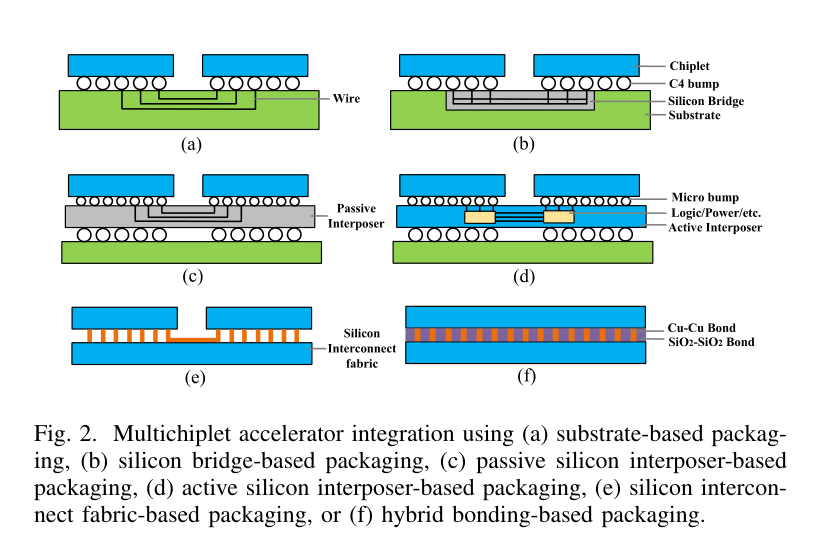
\includegraphics[width=0.88\textwidth]{chapters/ch09-chiplets-ucie/figures/chen_fig02_chiplet_packaging_taxonomy.png}
\caption{Packaging taxonomy for multi-chiplet architectures: (a) Standard organic substrate, (b) 2.5D silicon interposer (e.g., TSMC CoWoS), (c) Embedded bridge technology (e.g., Intel EMIB), and (d) 3D hybrid bonding. [Reproduced from: Z. Chen et al., ``HiRe: A Hierarchical Reconfigurable Architecture for Large-Scale Multichiplet DNN Accelerators'', \emph{IEEE Transactions on Very Large Scale Integration (VLSI) Systems}, Vol. 34, No. 4, pp. 880--893, 2026, DOI: 10.1109/TVLSI.2026.3676552.~\cite{Chen2026} \copyright\ 2026 IEEE]}
\label{fig:chen-chiplet-packaging}
\end{figure}

\subsection{Packaging Comparison \& Physical Trade-offs}

\begin{enumerate}
    \item \textbf{Standard Organic Substrate}: Chiplets are mounted directly onto a multi-layer printed circuit board (PCB) or organic laminate packaging substrate using standard flip-chip solder bumps (C4 bumps) with a pitch of $100\text{--}130\,\mu\mathrm{m}$. While low in cost, trace escape pitch constraints limit edge shoreline bandwidth density to $\approx 100\text{--}150\,\mathrm{Gbps/mm}$, and high trace capacitance results in energy dissipation of $1.0\text{--}1.5\,\mathrm{pJ/bit}$.
    
    \item \textbf{Passive Silicon Interposer (2.5D, CoWoS-S)}: Chiplets are micro-bumped onto a passive silicon carrier wafer containing fine-pitch copper interconnect wiring ($0.4\text{--}0.8\,\mu\mathrm{m}$ minimum metal pitch) and through-silicon vias. Micro-bump pitches range from $25\text{--}55\,\mu\mathrm{m}$, enabling shoreline bandwidth densities exceeding $700\text{--}1300\,\mathrm{Gbps/mm}$ at ultra-low energy dissipation ($0.2\text{--}0.4\,\mathrm{pJ/bit}$). However, the interposer size itself faces reticle limit constraints, requiring multi-reticle lithography stitching.
    
    \item \textbf{Embedded Silicon Bridges (EMIB)}: Instead of a full-size monolithic interposer, small localized silicon bridges containing ultra-fine-pitch wires are embedded inside the organic package beneath adjacent chiplet edges. This avoids the cost of a full silicon interposer while providing local micro-bump interconnect density.
    
    \item \textbf{Active Silicon Interposers}: In active interposers, the carrier silicon is not passive; it incorporates active CMOS transistors, integrated routers, network switches, and voltage regulators.
\end{enumerate}

\begin{figure}[htbp]
\centering
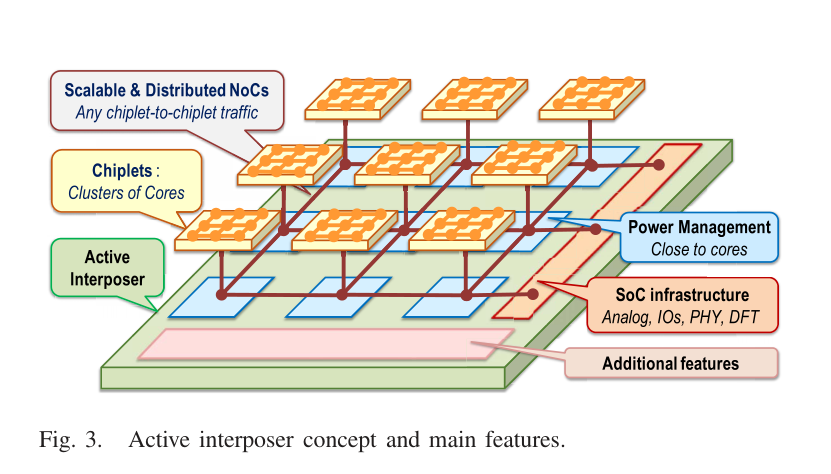
\includegraphics[width=0.88\textwidth]{chapters/ch09-chiplets-ucie/figures/vivet_fig03_active_interposer.png}
\caption{IntAct active interposer system architecture integrating six 16-core chiplets (96 cores total) over a 2D mesh active interposer NoC with integrated distributed power management. [Reproduced from: P. Vivet et al., ``IntAct: A 96-Core Processor With Six Chiplets 3D-Stacked on an Active Interposer With Distributed Interconnects and Integrated Power Management'', \emph{IEEE Journal of Solid-State Circuits}, Vol. 56, No. 1, pp. 79--97, Jan. 2021, DOI: 10.1109/JSSC.2020.3036341.~\cite{Vivet2021} \copyright\ 2021 IEEE]}
\label{fig:vivet-active-interposer}
\end{figure}

Fig.~\ref{fig:vivet-active-interposer} showcases the IntAct processor demonstrated by Vivet et al.~\cite{Vivet2021}. Six 16-core compute chiplets (each containing an $8 \times 2$ NoC tile array) are 3D-stacked via micro-bumps onto a large active interposer. The active interposer hosts a distributed $6 \times 4$ network-on-chip router fabric with asynchronous cross-die communication interfaces and on-chip DC-DC switched-capacitor voltage converters. This decouples compute-die routing from inter-chiplet global packet routing, achieving $3.0\,\mathrm{Tbps}$ cross-die bandwidth.

\section{The Universal Chiplet Interconnect Express (UCIe) Standard}
\label{sec:ucie-standard}

\begin{svgraybox}
\textbf{High-School Intuition: The Universal USB-C for Chiplets} \\
Can you plug an AMD compute chiplet into an Intel memory chiplet or an Apple graphics chiplet? Historically no, because each semiconductor company invented its own secret proprietary wires. The \textbf{Universal Chiplet Interconnect Express (UCIe)} standard acts as the universal ``USB-C'' standard for chiplets: an open industry rulebook that allows silicon tiles from any foundry in the world to connect and communicate seamlessly.
\end{svgraybox}

To prevent market fragmentation and proprietary interconnect lock-in, the open industry consortium established the \textbf{Universal Chiplet Interconnect Express (UCIe)} standard~\cite{UCIe2023}. UCIe provides a complete, standardized die-to-die interconnect stack partitioned into three hierarchical layers:

\begin{enumerate}
    \item \textbf{Protocol Layer}: Maps native standard high-level protocols into structured Flits (Flow Control Units). UCIe natively supports PCIe 6.0/7.0 for standard I/O attach, CXL 2.0/3.0 (\texttt{CXL.io}, \texttt{CXL.cache}, \texttt{CXL.mem}) for coherent shared-memory pooling, and user-defined Raw Streaming protocols for custom low-overhead NoC flit tunneling.
    
    \item \textbf{Die-to-Die (D2D) Adapter Layer}: Responsible for link state management, packet framing, cyclic redundancy check (CRC-16 or CRC-32) generation and checking, retry buffer management with link-level Go-Back-N or Selective Repeat retransmission, and flow control credit turnaround. It abstracts the physical signaling interface from the upper protocol stack.
    
    \item \textbf{Physical Layer (PHY)}: Implements electrical drivers, receivers, clock forwarders, lane training, deskew logic, and sideband control channels. UCIe defines two primary physical packaging profiles:
    \begin{itemize}
        \item \emph{Standard Package (UCIe-S)}: Targeted at standard organic substrates, utilizing single-ended signaling at data rates of $4\text{--}32\,\mathrm{Gbps/lane}$ across bump pitches of $100\text{--}130\,\mu\mathrm{m}$, achieving trace channel lengths up to $25\,\mathrm{mm}$.
        \item \emph{Advanced Package (UCIe-A)}: Targeted at silicon interposers, silicon bridges, and high-density fan-out substrates, utilizing micro-bump pitches of $25\text{--}55\,\mu\mathrm{m}$ with short channel lengths ($<2\text{--}3\,\mathrm{mm}$), achieving data rates up to $32\,\mathrm{Gbps/lane}$, shoreline bandwidth densities $>700\,\mathrm{Gbps/mm}$, and sub-$0.5\,\mathrm{pJ/bit}$ energy efficiency.
    \end{itemize}
\end{enumerate}

\section{Inter-Chiplet Latency, Bandwidth Density \& Credit Turnaround}
\label{sec:d2d-latency-credit}

\subsection{Round-Trip Latency Decomposition}

When a packet flit traverses a die-to-die chiplet boundary, it incurs latency contributions across multiple physical and protocol domains:
\begin{equation}
    t_{\mathrm{D2D}} = t_{\mathrm{CDC}} + t_{\mathrm{adapter}} + t_{\mathrm{PHY\_tx}} + t_{\mathrm{flight}} + t_{\mathrm{PHY\_rx}} + t_{\mathrm{deskew}} + t_{\mathrm{CDC}}
    \label{eq:d2d-latency}
\end{equation}
where:
\begin{itemize}
    \item $t_{\mathrm{CDC}}$ is the clock domain crossing synchronizer latency (typically 2 to 3 clock cycles of the receiving domain).
    \item $t_{\mathrm{adapter}}$ is the D2D adapter framing, CRC computation, and header generation latency (1 to 2 cycles).
    \item $t_{\mathrm{PHY\_tx}}$ and $t_{\mathrm{PHY\_rx}}$ denote serializer/deserializer and analog pad driving delays.
    \item $t_{\mathrm{flight}} = L_{\mathrm{channel}} / v_{\mathrm{prop}}$ is the physical propagation flight time along the interposer trace ($v_{\mathrm{prop}} \approx 1.5 \times 10^8\,\mathrm{m/s}$ in $\mathrm{SiO_2}$, yielding $\approx 6.7\,\mathrm{ps/mm}$).
    \item $t_{\mathrm{deskew}}$ represents the lane-to-lane phase alignment delay.
\end{itemize}

\subsection{Credit Turnaround \& Buffer Sizing}

To maintain peak line-rate throughput without stalling the transmitting chiplet, credit-based flow control requires sufficient buffer depth at the receiver. The round-trip turnaround time ($\mathrm{RTT}_{\mathrm{credit}}$) for a credit token is:
\begin{equation}
    \mathrm{RTT}_{\mathrm{credit}} = t_{\mathrm{forward}} + t_{\mathrm{rx\_process}} + t_{\mathrm{backward}} + t_{\mathrm{tx\_process}}
    \label{eq:credit-rtt}
\end{equation}
where $t_{\mathrm{forward}}$ is the forward flit latency, $t_{\mathrm{rx\_process}}$ is the receiver consumption and credit issue delay, $t_{\mathrm{backward}}$ is the reverse credit channel transmission delay, and $t_{\mathrm{tx\_process}}$ is the credit counter update time.

The minimum receiver buffer depth $B_{\mathrm{min}}$ (in flits) required to guarantee stall-free streaming is strictly bounded by Little's law:
\begin{equation}
    B_{\mathrm{min}} \ge \left\lceil \frac{\mathrm{RTT}_{\mathrm{credit}}}{T_{\mathrm{flit}}} \right\rceil = \left\lceil \mathrm{RTT}_{\mathrm{credit}} \cdot f_{\mathrm{clk}} \right\rceil
    \label{eq:credit-buffer}
\end{equation}
If $B < B_{\mathrm{min}}$, the transmitter exhausts its credit pool before receiving the return token, creating idle bubbled cycles on the high-bandwidth physical link.

\section{Deadlock in Multi-Chiplet Networks \& In/Outbound Swap Recovery}
\label{sec:chiplet-deadlocks}

\begin{svgraybox}
\textbf{High-School Intuition: The Four-Way Traffic Jam} \\
Imagine four cars arrive at an intersection at the same time: Car 1 waits for Car 2, Car 2 waits for Car 3, Car 3 waits for Car 4, and Car 4 waits for Car 1. Nobody can move! That is a routing deadlock. The \textbf{In/Outbound Swap} mechanism acts like a smart traffic cop: after detecting cars waiting too long ($\tau_{\mathrm{stall}}$), the cop tells Car 1 to pull into a side driveway (a 2-flit escape register). Instantly, Cars 4, 3, and 2 drive through! Then Car 1 rejoins the road. The jam is cleared with zero dropped packets.
\end{svgraybox}

\subsection{The Inter-Chiplet Deadlock Anomaly}

In monolithic 2D NoCs, routing deadlocks are prevented using standard turn models (e.g., XY Dimension-Order Routing, West-First, Odd-Even) that maintain an acyclic Channel Dependency Graph (CDG)~\cite{DallyPrinciples}. 

However, multi-chiplet systems are fundamentally \textbf{hierarchical networks}. Each individual chiplet typically runs an internal routing protocol (e.g., local 2D mesh DOR), while global traffic between chiplets is handled by bridge routers connected across D2D links. 

As proved by Wang et al.~\cite{Wang2026}, composition of deadlock-free local networks does \emph{not} guarantee global deadlock-freedom. Cyclic buffer dependencies emerge across chiplet boundaries due to turn combination loops and mismatched D2D bridge queue capacities, as illustrated in Fig.~\ref{fig:wang-deadlock-subpath}.

\begin{figure}[htbp]
\centering
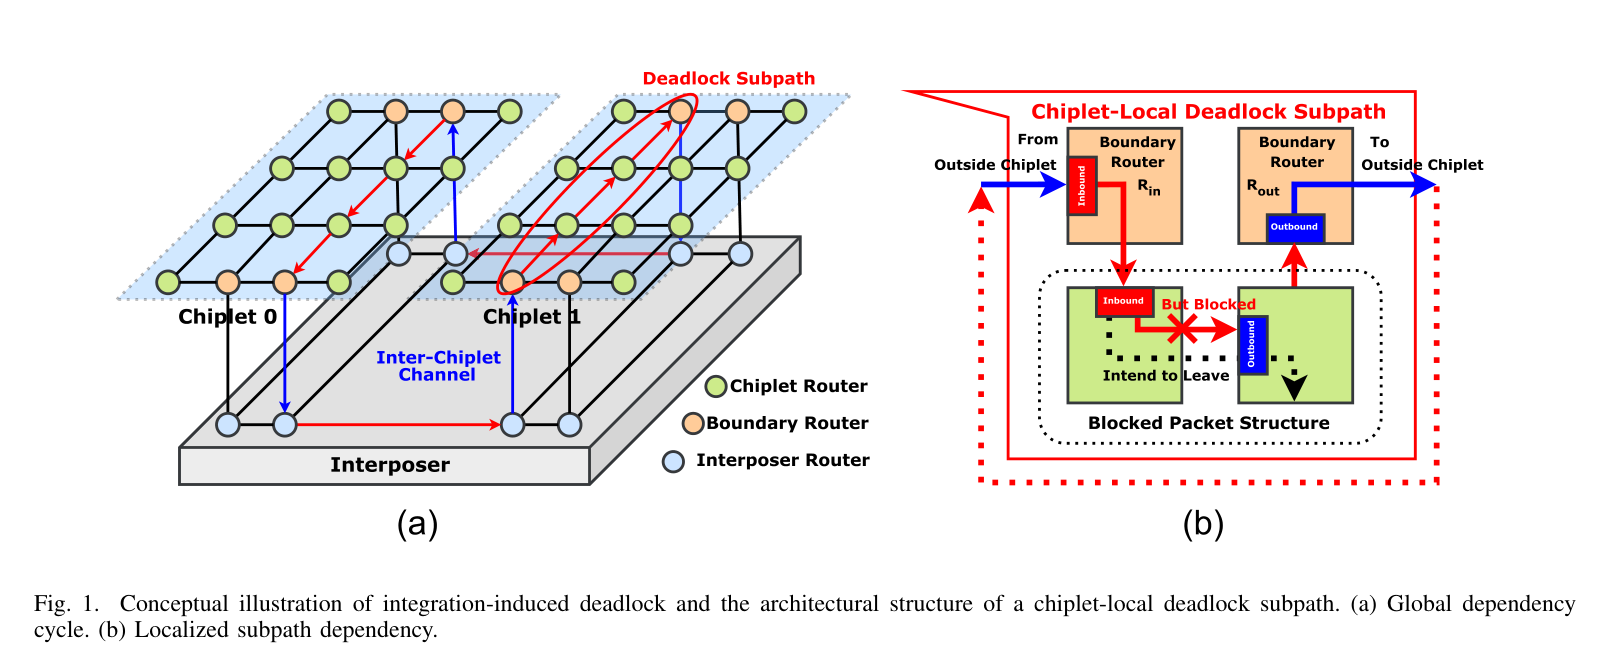
\includegraphics[width=0.88\textwidth]{chapters/ch09-chiplets-ucie/figures/wang_fig01_chiplet_deadlock_subpath.png}
\caption{Multi-chiplet routing deadlock scenario where local subpath dependencies cross die-to-die bridge boundaries, forming a closed resource dependency cycle across Chiplet 1, Chiplet 2, Chiplet 3, and Chiplet 4. [Reproduced from: P. Wang et al., ``In/Outbound Swap: A Backtracking-based Deadlock Recovery Mechanism for Multi-Chiplet Networks'', \emph{IEEE Transactions on Computer-Aided Design of Integrated Circuits and Systems}, Vol. 45, No. 5, pp. 2100--2114, 2026, DOI: 10.1109/TCAD.2026.3688573.~\cite{Wang2026} \copyright\ 2026 IEEE]}
\label{fig:wang-deadlock-subpath}
\end{figure}

\subsection{Deadlock Avoidance vs. Recovery}

There are two primary paradigms to address multi-chiplet deadlocks:
\begin{enumerate}
    \item \textbf{Deadlock Avoidance via Dedicated Virtual Channels}: Dedicating separate virtual channels (VCs) for local intra-chiplet flits, inter-chiplet outbound flits, and inbound transit flits. While mathematically acyclic, this approach imposes severe buffer area overheads (doubling or tripling input FIFO queues at every bridge router) and degrades VC buffer utilization during non-congested execution.
    
    \item \textbf{Deadlock Recovery via Backtracking (In/Outbound Swap)}: Wang et al.~\cite{Wang2026} proposed the \textbf{In/Outbound Swap} mechanism. Instead of allocating costly redundant VCs, the network operates dynamically with minimal buffers. When a cyclic stall is detected at a bridge router boundary, stalled packets are systematically backtracked and swapped between inbound and outbound escape queues, untangling the dependency loop without dropping flits.
\end{enumerate}

\begin{figure}[htbp]
\centering
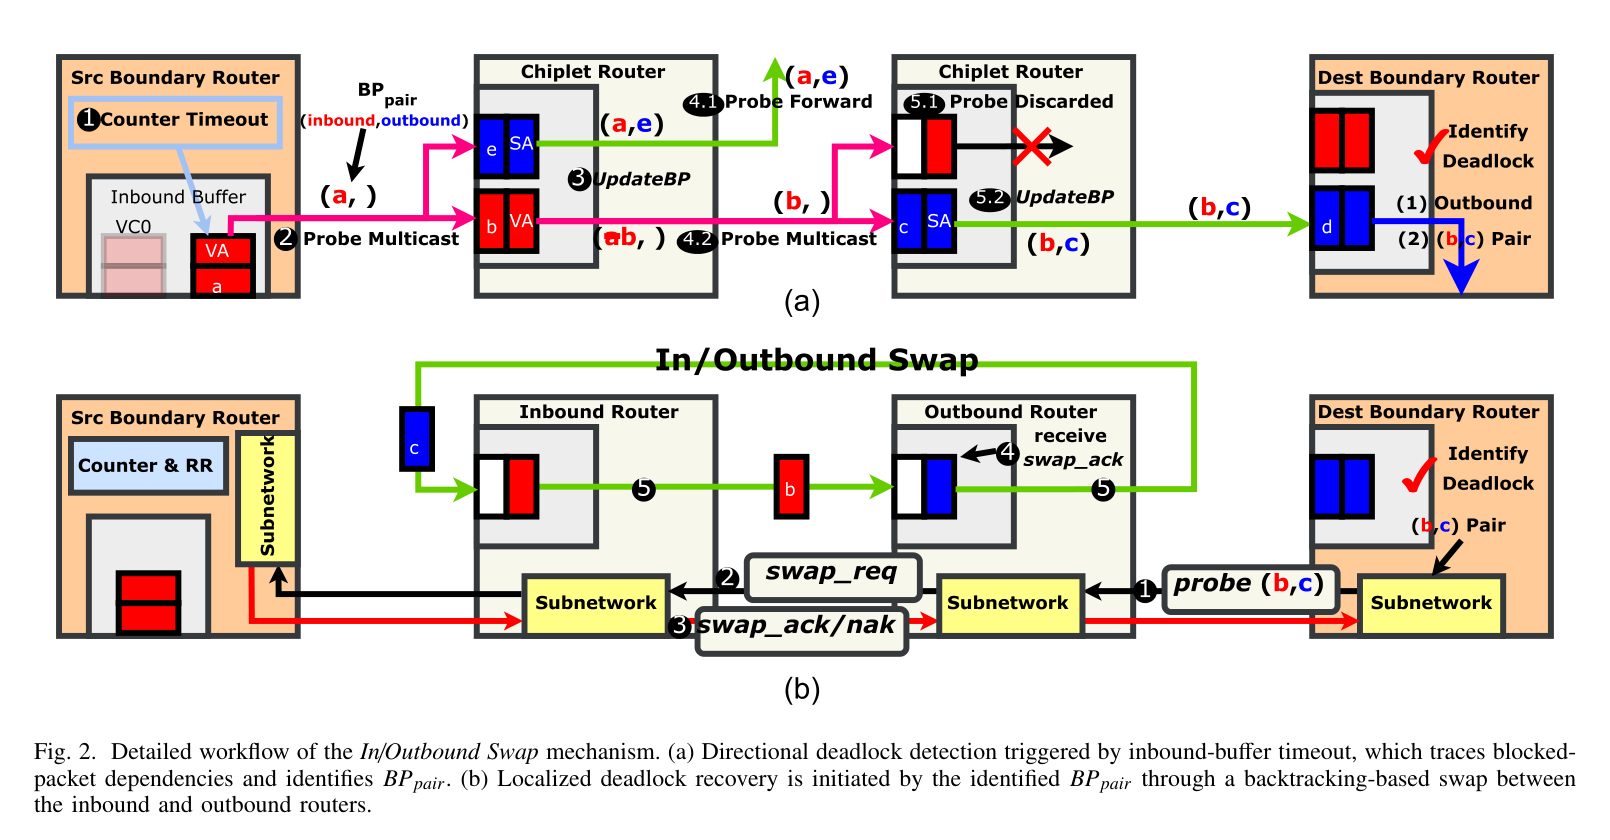
\includegraphics[width=0.88\textwidth]{chapters/ch09-chiplets-ucie/figures/wang_fig02_swap_recovery_flow.png}
\caption{Operational flow of the In/Outbound Swap deadlock recovery mechanism: stall timeout detection, swap request assertion, queue handshake, and circular dependency breaking. [Reproduced from: P. Wang et al., ``In/Outbound Swap: A Backtracking-based Deadlock Recovery Mechanism for Multi-Chiplet Networks'', \emph{IEEE Transactions on Computer-Aided Design of Integrated Circuits and Systems}, Vol. 45, No. 5, pp. 2100--2114, 2026, DOI: 10.1109/TCAD.2026.3688573.~\cite{Wang2026} \copyright\ 2026 IEEE]}
\label{fig:wang-swap-flow}
\end{figure}

As depicted in Fig.~\ref{fig:wang-swap-flow}, the In/Outbound Swap architecture incorporates a threshold stall counter ($\tau_{\mathrm{stall}}$) at each D2D bridge interface. If a head flit remains blocked at the inter-chiplet output port for more than $\tau_{\mathrm{stall}}$ cycles while downstream credits remain zero, a potential deadlock cycle is flagged. The bridge controller triggers a bidirectional handshake across the D2D interface, rerouting the stalled head flit into a dedicated 2-flit swap escape register. This releases the upstream input port, enabling trailing flits from non-deadlocked flows to advance. Once the dependency cycle is broken, normal credit flow resumes.

\section{Hardware Implementation: Chiplet D2D Bridge Controller}
\label{sec:chiplet-verilog}

Listing~\ref{lst:chiplet-bridge-verilog} shows the synthesizable Verilog implementation of an inter-chiplet bridge protocol controller with dual-clock asynchronous FIFO synchronization, credit-based flow control, CRC-8 error monitoring, and the In/Outbound Swap deadlock recovery mechanism.

\begin{lstlisting}[language=Verilog, caption={Synthesizable Multi-Chiplet D2D Bridge Protocol Controller with In/Outbound Swap Recovery (\texttt{chiplet\_bridge\_protocol.v})}, label={lst:chiplet-bridge-verilog}]
module chiplet_bridge_protocol #(
    parameter DATA_WIDTH     = 64,
    parameter FIFO_DEPTH     = 16,
    parameter ADDR_WIDTH     = 4,
    parameter STALL_TIMEOUT  = 64
)(
    // Local Chiplet Clock & Reset
    input  wire                  local_clk,
    input  wire                  local_rst_n,

    // Local Inbound NoC Interface
    input  wire [DATA_WIDTH-1:0] tx_flit_data,
    input  wire                  tx_flit_valid,
    output wire                  tx_flit_ready,

    // Local Outbound NoC Interface
    output reg  [DATA_WIDTH-1:0] rx_flit_data,
    output reg                   rx_flit_valid,
    input  wire                  rx_flit_ready,

    // Die-to-Die (D2D) Physical Interface (Remote Clock)
    input  wire                  d2d_rx_clk,
    input  wire                  d2d_rx_rst_n,
    input  wire [DATA_WIDTH-1:0] d2d_rx_data,
    input  wire                  d2d_rx_valid,
    input  wire [7:0]            d2d_rx_crc,
    output wire                  d2d_rx_credit,

    // D2D Transmit Interface (Local Clock forward)
    output reg  [DATA_WIDTH-1:0] d2d_tx_data,
    output reg                   d2d_tx_valid,
    output reg  [7:0]            d2d_tx_crc,
    input  wire                  d2d_tx_credit,

    // Deadlock Swap Recovery Signals
    output reg                   swap_active,
    output reg                   deadlock_detected
);

    // Credit Counter for Remote D2D Receiver
    reg [ADDR_WIDTH:0] d2d_tx_credits;
    wire has_tx_credit = (d2d_tx_credits > 0);

    // Stall Timer for Deadlock Detection
    reg [15:0] stall_counter;
    reg [DATA_WIDTH-1:0] swap_buffer;
    reg swap_buffer_valid;

    // CRC-8 Generation Function (x^8 + x^2 + x + 1)
    function [7:0] crc8_calc(input [DATA_WIDTH-1:0] data);
        integer b;
        reg [7:0] c;
        begin
            c = 8'hFF;
            for (b = 0; b < DATA_WIDTH; b = b + 1) begin
                if ((c[7] ^ data[b]) == 1'b1)
                    c = (c << 1) ^ 8'h07;
                else
                    c = c << 1;
            end
            crc8_calc = c;
        end
    endfunction

    // Transmit & Stall Monitoring FSM
    always @(posedge local_clk or negedge local_rst_n) begin
        if (!local_rst_n) begin
            d2d_tx_data       <= {DATA_WIDTH{1'b0}};
            d2d_tx_valid      <= 1'b0;
            d2d_tx_crc        <= 8'h00;
            d2d_tx_credits    <= FIFO_DEPTH;
            stall_counter     <= 16'd0;
            swap_active       <= 1'b0;
            deadlock_detected <= 1'b0;
            swap_buffer_valid <= 1'b0;
            swap_buffer       <= {DATA_WIDTH{1'b0}};
        end else begin
            // Credit management
            if (d2d_tx_credit && !d2d_tx_valid)
                d2d_tx_credits <= d2d_tx_credits + 1'b1;
            else if (!d2d_tx_credit && d2d_tx_valid && has_tx_credit)
                d2d_tx_credits <= d2d_tx_credits - 1'b1;

            // In/Outbound Swap Deadlock Recovery Trigger
            if (tx_flit_valid && !has_tx_credit) begin
                stall_counter <= stall_counter + 1'b1;
                if (stall_counter >= STALL_TIMEOUT) begin
                    deadlock_detected <= 1'b1;
                    swap_active       <= 1'b1;
                    // Latch blocked flit into swap escape register
                    swap_buffer       <= tx_flit_data;
                    swap_buffer_valid <= 1'b1;
                end
            end else begin
                stall_counter     <= 16'd0;
                deadlock_detected <= 1'b0;
            end

            // Packet transmission
            if (has_tx_credit && (tx_flit_valid || swap_buffer_valid)) begin
                if (swap_buffer_valid) begin
                    d2d_tx_data       <= swap_buffer;
                    d2d_tx_crc        <= crc8_calc(swap_buffer);
                    d2d_tx_valid      <= 1'b1;
                    swap_buffer_valid <= 1'b0;
                    swap_active       <= 1'b0;
                end else begin
                    d2d_tx_data       <= tx_flit_data;
                    d2d_tx_crc        <= crc8_calc(tx_flit_data);
                    d2d_tx_valid      <= 1'b1;
                end
            end else begin
                d2d_tx_valid <= 1'b0;
            end
        end
    end

    assign tx_flit_ready = has_tx_credit && !swap_buffer_valid;

    // Receive Logic with CRC Checking
    reg credit_return_pulse;
    assign d2d_rx_credit = credit_return_pulse;

    always @(posedge d2d_rx_clk or negedge d2d_rx_rst_n) begin
        if (!d2d_rx_rst_n) begin
            rx_flit_data        <= {DATA_WIDTH{1'b0}};
            rx_flit_valid       <= 1'b0;
            credit_return_pulse <= 1'b0;
        end else begin
            if (d2d_rx_valid && (crc8_calc(d2d_rx_data) == d2d_rx_crc)) begin
                rx_flit_data        <= d2d_rx_data;
                rx_flit_valid       <= 1'b1;
                credit_return_pulse <= 1'b1; // Acknowledge credit return
            end else begin
                rx_flit_valid       <= 1'b0;
                credit_return_pulse <= 1'b0;
            end
        end
    end
endmodule
\end{lstlisting}

\section{Simulation Model \& Quantitative Evaluation}
\label{sec:chiplet-sim-results}

To evaluate D2D packaging trade-offs quantitatively, the accompanying Python model \texttt{ucie\_d2d\_latency\_model.py} analyzes latency, bandwidth, power, and credit requirements for standard organic packages versus advanced 2.5D silicon interposers. Table~\ref{tab:chiplet-pkg-eval} summarizes the comparative performance metrics.

\begin{table}[htbp]
\centering
\caption{Quantitative Packaging Comparison: Standard Organic vs. Advanced Silicon Interposer (UCIe)}
\label{tab:chiplet-pkg-eval}
\begin{tabular}{lcc}
\hline
\textbf{Metric} & \textbf{Standard Organic} & \textbf{Advanced Silicon Interposer} \\
\hline
Bump / Pad Pitch & $110\,\mu\mathrm{m}$ & $\mathbf{45\,\mu\mathrm{m}}$ \\
Trace Channel Length & $15.0\,\mathrm{mm}$ & $\mathbf{1.8\,\mathrm{mm}}$ \\
Forward Propagation Delay & $100.0\,\mathrm{ps}$ & $\mathbf{12.0\,\mathrm{ps}}$ \\
Clock Frequency & $2.0\,\mathrm{GHz}$ & $\mathbf{2.0\,\mathrm{GHz}}$ \\
One-Way Latency ($t_{\mathrm{D2D}}$) & $4.25\,\mathrm{ns}$ ($8.5\,\mathrm{cycles}$) & $\mathbf{4.06\,\mathrm{ns}}$ ($8.1\,\mathrm{cycles}$) \\
Credit Round-Trip Time ($\mathrm{RTT}_{\mathrm{credit}}$) & $8.50\,\mathrm{ns}$ ($17.0\,\mathrm{cycles}$) & $\mathbf{8.11\,\mathrm{ns}}$ ($16.2\,\mathrm{cycles}$) \\
Minimum Buffer Depth ($B_{\mathrm{min}}$) & $17\,\mathrm{flits}$ & $\mathbf{17\,\mathrm{flits}}$ \\
Total Raw Bandwidth & $0.51\,\mathrm{Tbps}$ ($64.0\,\mathrm{GB/s}$) & $\mathbf{2.05\,\mathrm{Tbps}}$ ($256.0\,\mathrm{GB/s}$) \\
Shoreline Bandwidth Density & $145.5\,\mathrm{Gbps/mm}$ & $\mathbf{711.1\,\mathrm{Gbps/mm}}$ ($4.88\times$) \\
Energy Efficiency & $1.200\,\mathrm{pJ/bit}$ & $\mathbf{0.330\,\mathrm{pJ/bit}}$ ($3.64\times\text{ lower}$) \\
Total Interface Power & $614.4\,\mathrm{mW}$ & $\mathbf{675.8\,\mathrm{mW}}$ \\
Protocol Framing Yield & $91.2\%$ & $\mathbf{97.7\%}$ \\
\hline
\end{tabular}
\end{table}

The simulation highlights the decisive advantages of advanced silicon interposers. With a bump pitch of $45\,\mu\mathrm{m}$, the advanced interposer delivers $711.1\,\mathrm{Gbps/mm}$ linear shoreline bandwidth density—a $4.88\times$ improvement over standard organic laminate substrates. Crucially, its shorter trace length ($1.8\,\mathrm{mm}$ vs. $15.0\,\mathrm{mm}$) and reduced capacitive loading drive energy dissipation down to $0.33\,\mathrm{pJ/bit}$, enabling terabit-per-second die-to-die communication within strict power envelopes.

\section{Summary}
\label{sec:ch9_summary}

This chapter explored the physical, architectural, and protocol foundations of multi-chiplet interconnects and 2.5D systems. By modularizing large monolithic dies into cost-effective chiplets, systems overcome optical reticle boundaries and defect density yield limitations. Advanced silicon interposers and embedded bridges provide shoreline bandwidth densities approaching $1\,\mathrm{Tbps/mm}$ at sub-$0.5\,\mathrm{pJ/bit}$ energy metrics. The UCIe specification formalizes physical, adapter, and protocol layering, ensuring robust interoperability. Finally, the In/Outbound Swap backtracking mechanism resolves inter-die routing deadlocks dynamically, circumventing expensive buffer overprovisioning.

\section{Exercises and Review Questions}
\label{sec:ch9_exercises}

\begin{enumerate}
    \item \textbf{Die Yield and Cost Economics}: Consider a computing system requiring $800\,\mathrm{mm^2}$ of total silicon area. Assume a wafer diameter of $300\,\mathrm{mm}$, defect density $D_0 = 0.08\,\mathrm{defects/cm^2}$, wafer cost $C_{\mathrm{wafer}} = \$12{,}000$, and packaging cost $C_{\mathrm{pkg}} = \$80$ for monolithic vs. $\$160$ for a 4-chiplet 2.5D interposer assembly.
    \begin{enumerate}
        \item Using Murphy's model $Y = ((1 - e^{-A \cdot D_0})/(A \cdot D_0))^2$, calculate the yield of a monolithic $800\,\mathrm{mm^2}$ die ($A = 8.0\,\mathrm{cm^2}$).
        \item Calculate the yield of four independent $200\,\mathrm{mm^2}$ chiplets ($A = 2.0\,\mathrm{cm^2}$).
        \item Compute the net cost per good tested system for monolithic versus chiplet packaging.
    \end{enumerate}

    \item \textbf{Credit Queue Sizing for D2D Interfaces}: A UCIe-Advanced die-to-die link operates at a core clock frequency of $2.5\,\mathrm{GHz}$ ($T_{\mathrm{clk}} = 0.4\,\mathrm{ns}$). The transmitter adapter has a framing delay of $1.2\,\mathrm{ns}$, the PHY driver delay is $0.8\,\mathrm{ns}$, the interposer flight time is $0.2\,\mathrm{ns}$, the receiver deskew delay is $0.6\,\mathrm{ns}$, and CDC synchronization consumes 2 receiving clock cycles. The reverse credit channel requires identical latency.
    \begin{enumerate}
        \item Calculate the total one-way forward latency $t_{\mathrm{forward}}$.
        \item Calculate the total credit round-trip time $\mathrm{RTT}_{\mathrm{credit}}$.
        \item Determine the minimum number of buffer flits ($B_{\mathrm{min}}$) required to prevent link idling.
    \end{enumerate}

    \item \textbf{Deadlock Formation in Hierarchical Networks}: Prove why composing two deadlock-free 2D mesh networks using XY Dimension-Order Routing via a bidirectional inter-chiplet bridge link can produce a cyclic channel dependency if packets make turns between local and global channels.

    \item \textbf{In/Outbound Swap Deadlock Recovery}: Explain how the In/Outbound Swap mechanism breaks the four Coffman deadlock conditions (mutual exclusion, hold and wait, no preemption, and circular wait). Which specific condition is violated when a blocked packet is diverted into the swap escape register?
\end{enumerate}
